\begin{figure}
	\centering
	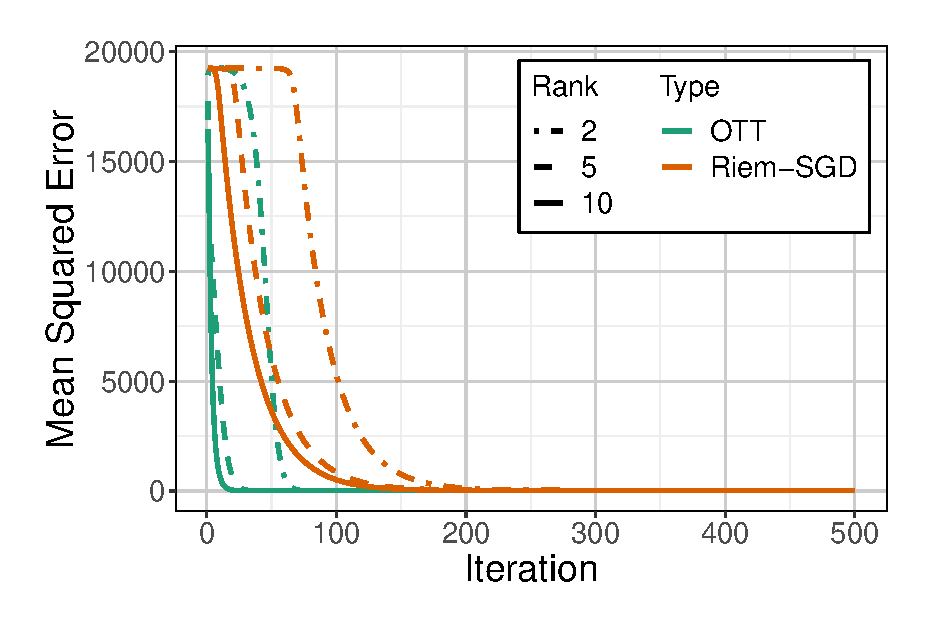
\includegraphics[width=0.32\textwidth]{4_ott/figs/sim/rank_convergence.eps}
	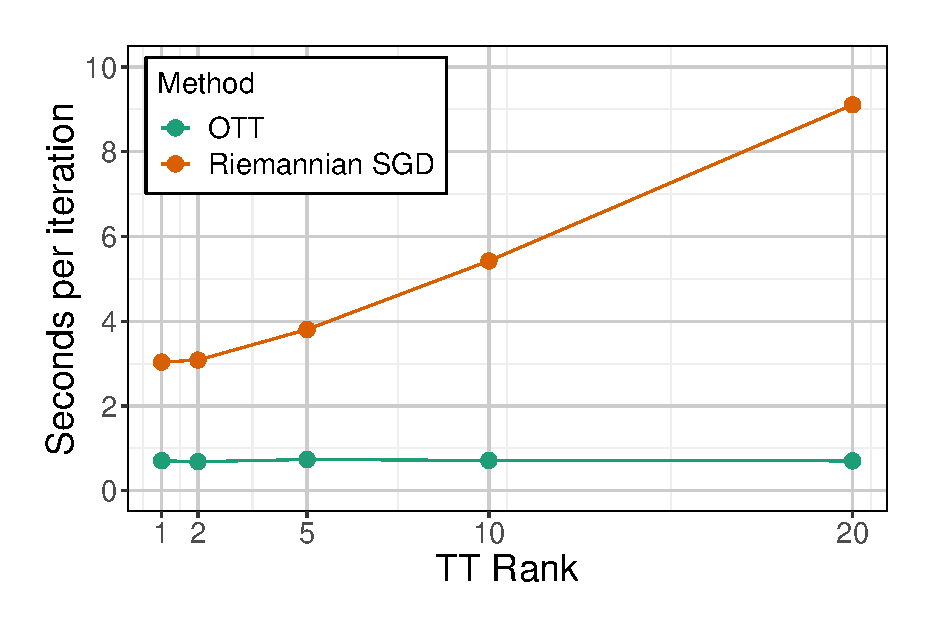
\includegraphics[width=0.32\textwidth]{4_ott/figs/sim/time_comparison.eps}
    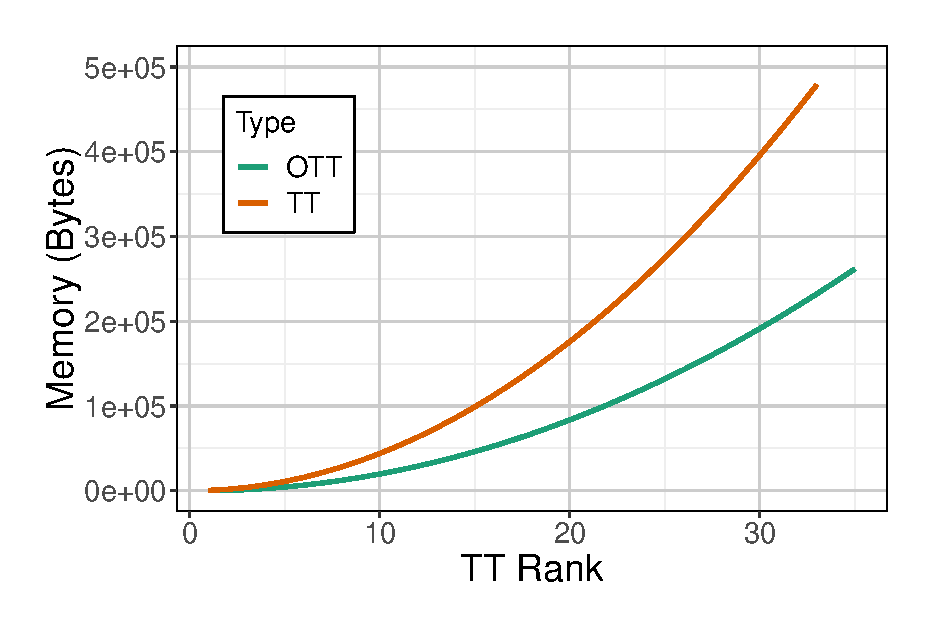
\includegraphics[width=0.32\textwidth]{4_ott/figs/sim/mem_vs_rank.eps}
	\caption{\label{fig:riemstief} \footnotesize (left) Mean squared error for different TT-ranks,
          using both the Riemannian formulation \eqref{eq:riem} and the approximate Stiefel formulation \eqref{eq:eott}.
          (center) Effect of TT-rank on per iteration runtime of both methods. OTT is significantly faster (10x)
          than the Riemannian formulation.
          (right) Memory Dependence of both TT and OTT constructions as a function of rank.
          The OTT formulation allows for models roughly double the size of TT.}
\end{figure}

\section{Evaluating performance on Simulations, Moving MNIST and Video data}\label{sec:exps}
First,
we evaluate how well our OTT formulation performs relative to existing methods, on synthetic
datasets as well as other popular datasets used for sequential deep models. 
%All synthetic experiments were conducted using a Tensorflow implementation on
A Nvidia Titan Xp GPU was used. 

\textbf{(A) OTT vs Riemannian SGD on synthetic data.}
To empirically verify the claims in Section \ref{sec:ott}
and to evaluate the value of our OTT construction over the existing Riemannian SGD framework,
we simulate a simple least squares problem with the goal of learning a tensorized weight matrix,
$$\min_{W_{TT}} \sum_{i=1}^n ||y_i - W_{TT}x_i||^.2$$
Here we use the na\"ive but exact OTT construction,
using the optimization scheme in Section \ref{sec:opt}.
A weight matrix $W$ is initialized to a random matrix with size $784 \times 625$, and samples are drawn from $y=Wx$. The matrix is reshaped as a tensor with modes $[4,7,4,7] \times [5,5,5,5]$.

\paragraph{Results.} Figure \ref{fig:riemstief} shows the
convergence rates of both methods with fixed learning rates for various TT-ranks.
\textbf{(a) Quality and speed.} For this toy problem, not only is the OTT construction able to find a good solution, it is able to find it significantly faster than Riemannian SGD.
\textbf{(b) Update steps.} Additionally, we note that the time per iteration is significantly shorter for the OTT construction.
%On the hardware described the OTT method takes approximately 0.07 seconds/iteration, while the Riemannian method takes 0.38, 0.55, and 1.00 seconds per iteration for each of the TT ranks evaluated.
OTT allows for each manifold update step to be performed on a low dimensional Stiefel,
and so retraction and projection is \textit{fast.}
The Riemannian method requires left orthogonalization and QR decompositions
of larger matrices, leading to a slower, TT-rank dependent runtime, shown in Figure \ref{fig:riemstief}.
\textbf{(c) Memory footprint.} Finally, we see in Figure \ref{fig:riemstief} that the memory consumption of OTT is quite modest compared to TT (which already offers
significant memory savings over alternative existing schemes). This may be a beneficial feature
when running a large sequential model on less expensive GPUs. 
Given these results, we use a basic SGD update for TT in subsequent experiments. 

\paragraph{(B) Moving MNIST.}
The moving MNIST dataset \cite{srivastava2015unsupervised} consists of handwritten digits moving within a specified larger image.
%Designed as a toy version of video data, moving MNIST is a standard benchmark for recurrent algorithms.
We first demonstrate that
for simple sequences, reconstruction under a complete tensor train framework is possible,
and representing fully connected layers with an OTT layer
reduces the number of parameters \textbf{without} image degradation.
Here, we use a vanilla RNN, with a state size of 4096 and TT-Rank 64.
%Figure \ref{fig:ttvsottmnist} shows the outputs after 100 training epochs of 20K samples with a batch size of 32. The hidden layer was of size 1024 and TT-rank 32, for images of size $64 \times 64$. Comparing the TT and OTT results, we observe a slight difference in reconstruction quality, at the cost of a hidden layer twice as large.
%\begin{figure*}[t]
%    \centering
%    $\overbrace{\hspace{0.495\textwidth}}^{\text{OTT Reconstruction}}$ $\overbrace{\hspace{0.495\textwidth}}^{\text{TT Reconstruction}}$ \\
%    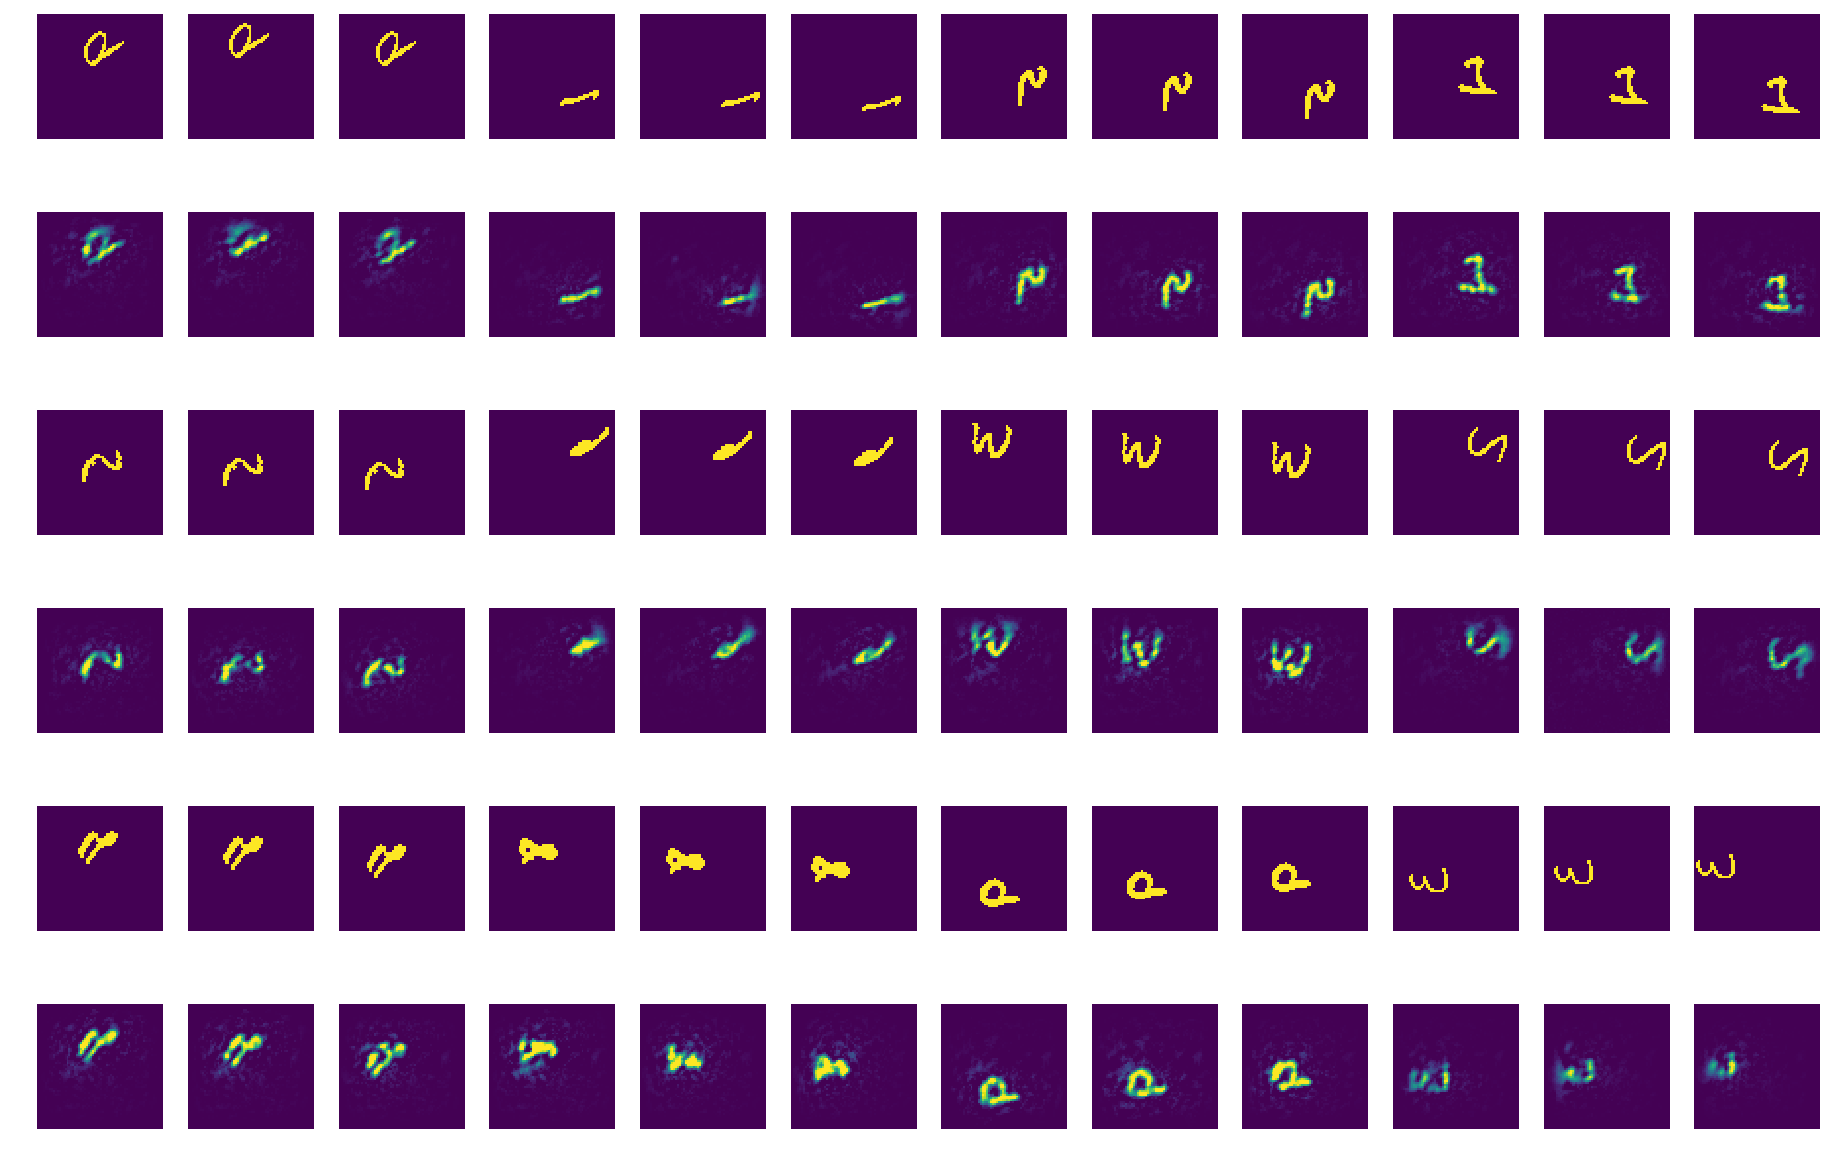
\includegraphics[width=0.49\textwidth,trim={24cm 20cm 0 0},clip]{figs/ott_epoch_99_valid_imgs.png}
%    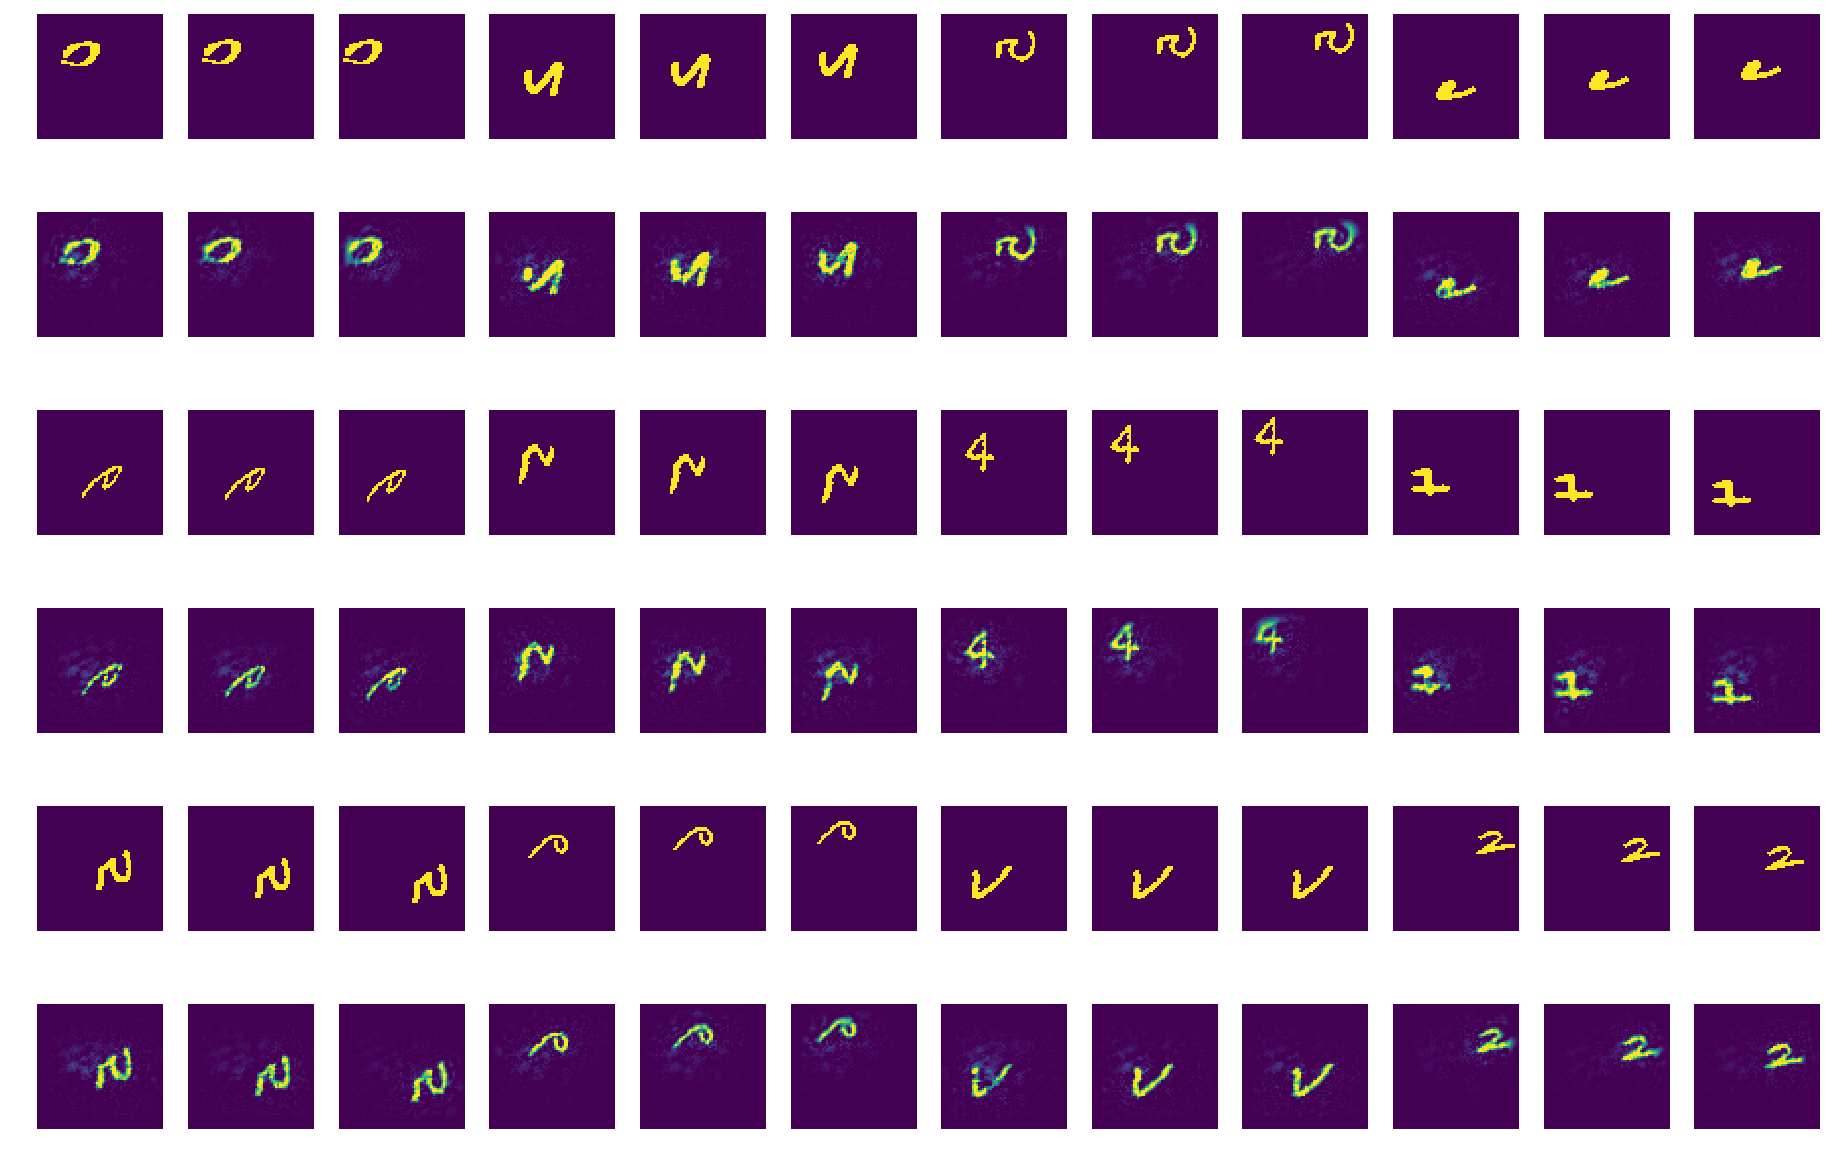
\includegraphics[width=0.49\textwidth,trim={24cm 0 0 20cm},clip]{figs/tt_epoch_99_valid_imgs.png}
%    \caption{Reconstruction results of 3-length Moving MNIST digits with frame size 64 by 64 pixels, for both TT and OTT constructions.}
%    \label{fig:ttvsottmnist}
%\end{figure*}

\paragraph{Results.} Figure \ref{fig:256digits} shows the ground truth and reconstruction
results for images with size $256 \times 256$, where each sequence is of length 8,
and the direction and orientation of the digit is random.
\textbf{(a) Reconstruction accuracy and model size.}
The entire recurrent network is compressed with OTT layers for input-to-hidden, hidden-to-hidden,
and hidden-to-output maps. With a large state size of 4096, we are able to nicely capture and
rebuild the entire sequence with a significantly smaller model size.
\begin{figure}
    \centering
    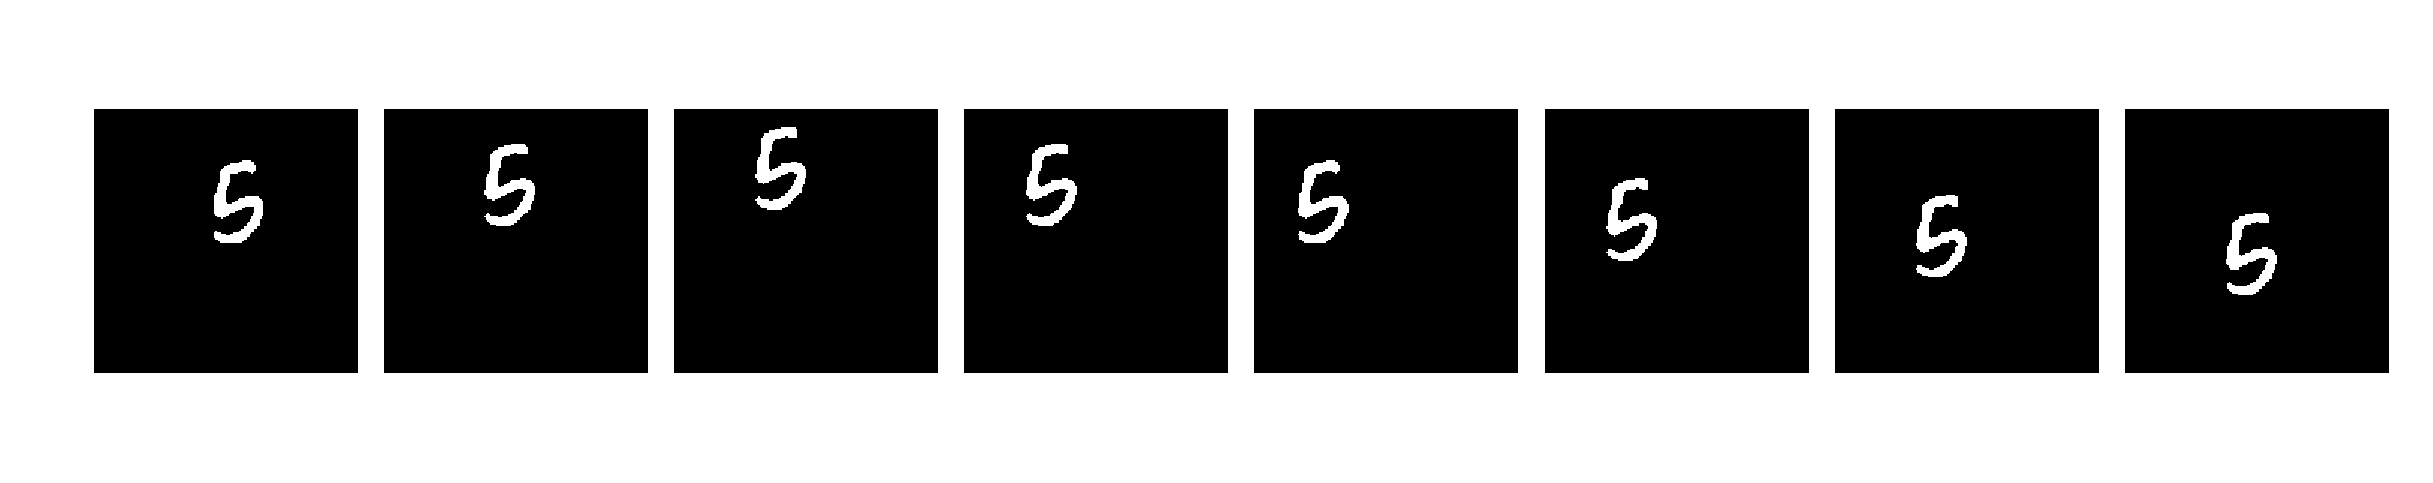
\includegraphics[width=0.9\textwidth,trim={0 1.5cm 0 1cm},clip]{4_ott/figs/mnist/DMNIST_gt.eps}
    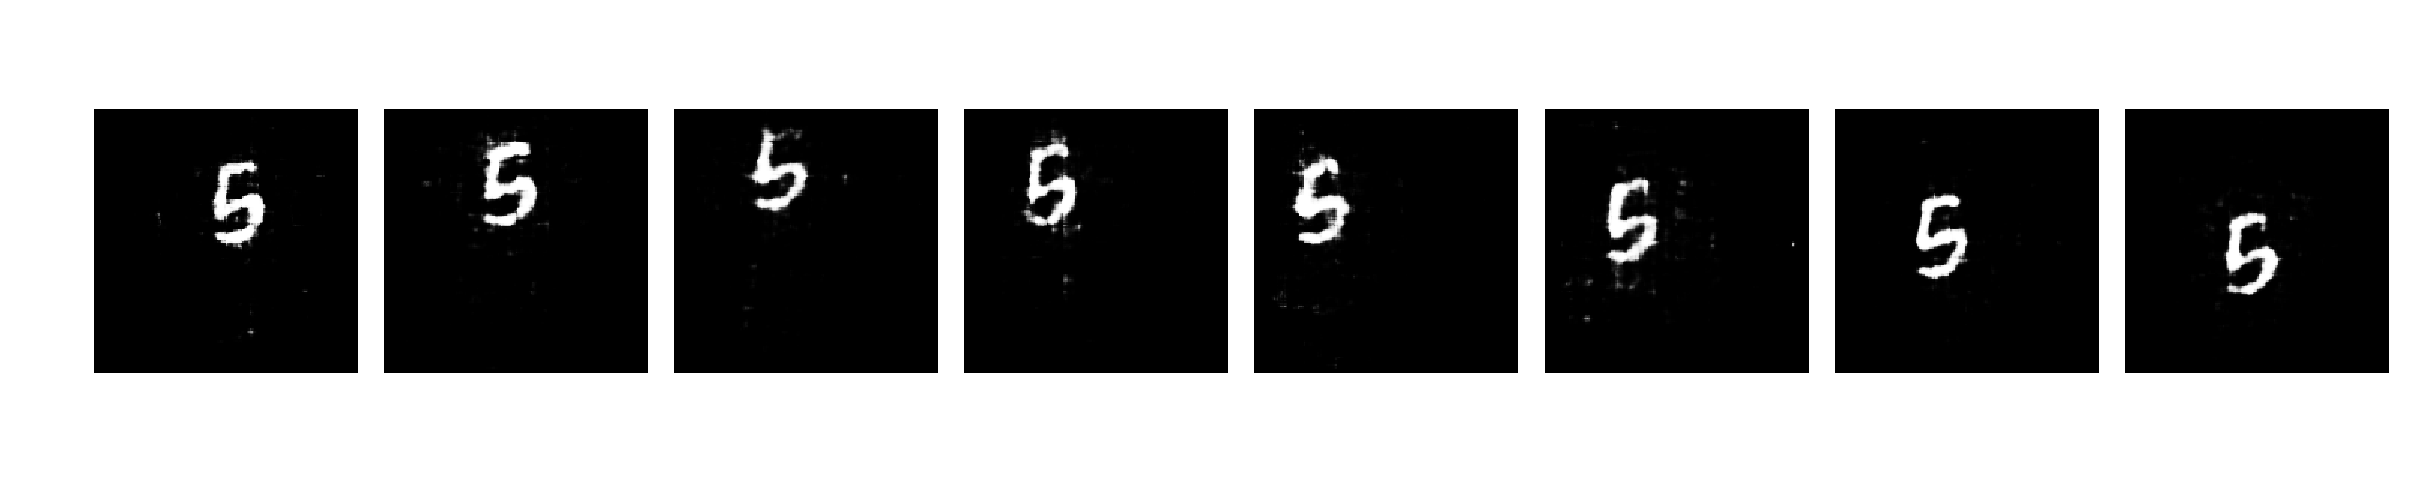
\includegraphics[width=0.9\textwidth,trim={0 1cm 0 1.5cm},clip]{4_ott/figs/mnist/DMNIST_pd.eps}
    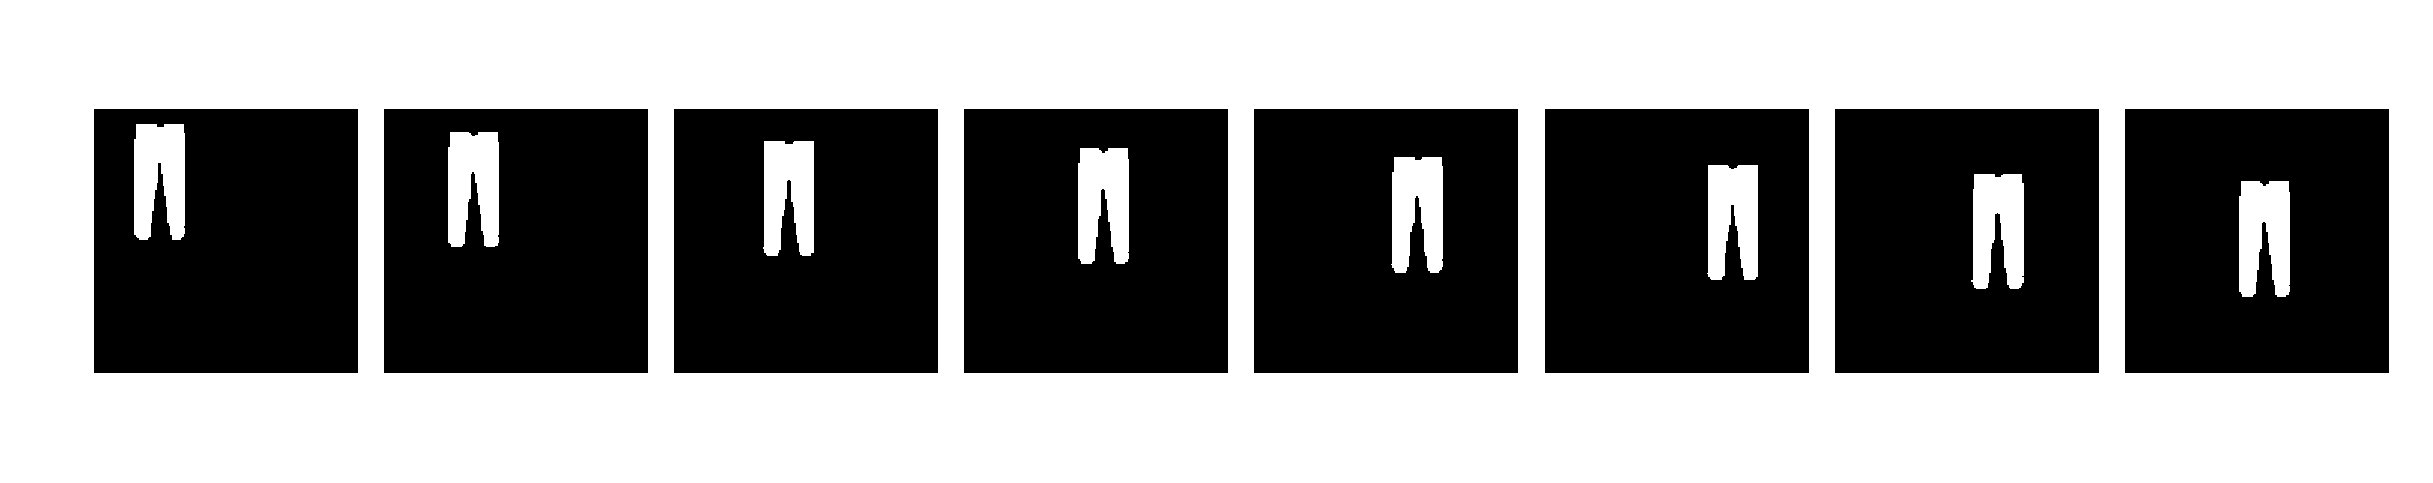
\includegraphics[width=0.9\textwidth,trim={0 1.5cm 0 1cm},clip]{4_ott/figs/mnist/FMNIST_gt.eps}
    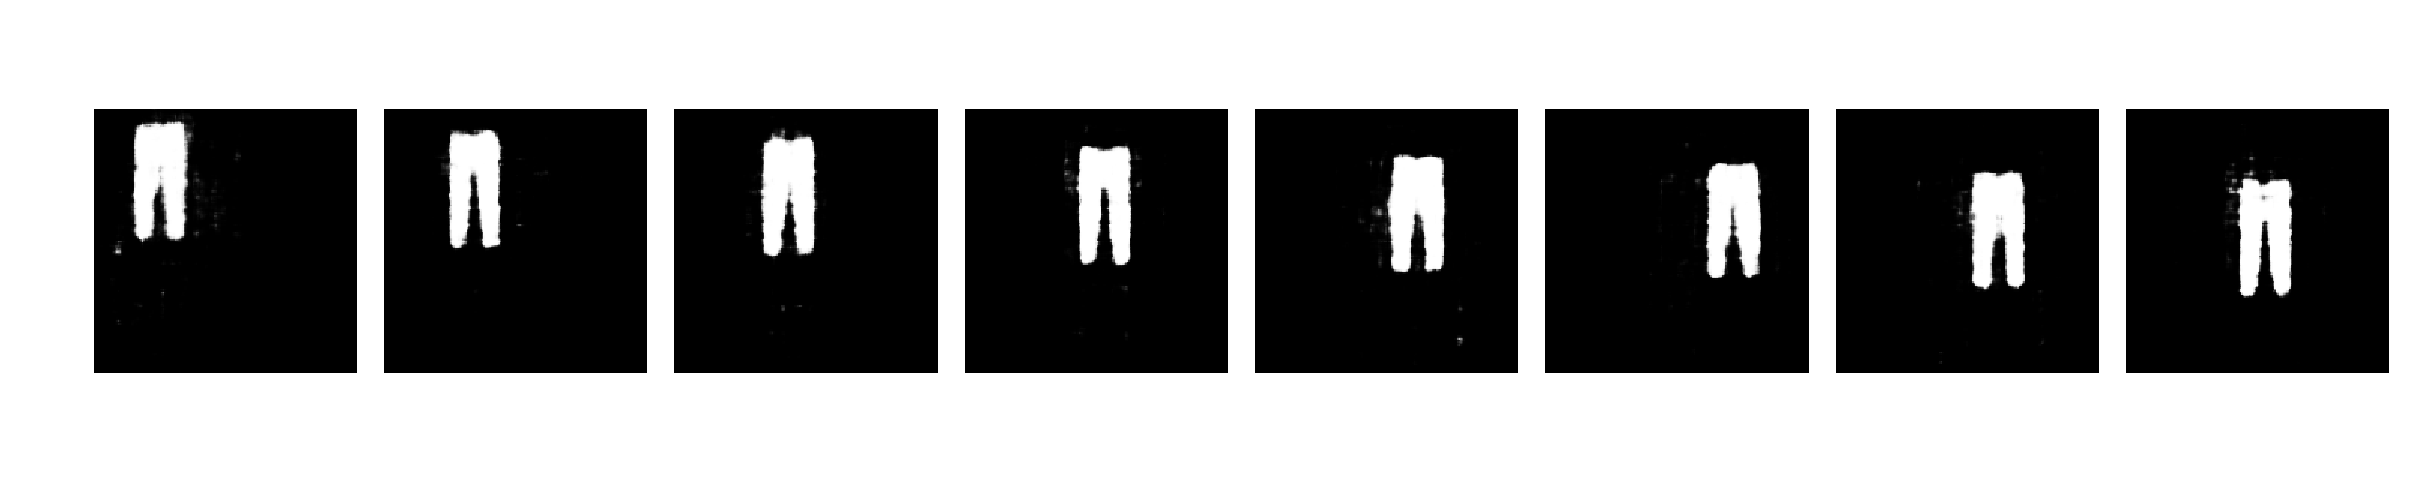
\includegraphics[width=0.9\textwidth,trim={0 1cm 0 1.5cm},clip]{4_ott/figs/mnist/FMNIST_pd.eps}
    \vspace{-10pt}
    \caption{    \label{fig:256digits} \footnotesize Sample ground truth (top) and reconstruction (bottom) of Moving MNIST digit and fashion sequences of size $256 \times 256$. We
    see good consistency between each upper/lower rows for both datasets.}
\end{figure}
\textbf{(b) Scaling to larger images.}
This effective compression also allows us to scale up --  to
significantly larger images of size $1024 \times 1024$, \textit{with no loss in reconstruction quality},
    without the need for more sophisticated convolutional architectures.

\textbf{(C) Hollywood2.}
We find
    that these results extend nicely to LSTMs/GRUs and for classification tasks
    as well. The Hollywood2 dataset \cite{marszalek09} consists of video clips from 69 movies
    labeled with 12 different actions from ``answering the phone" to ``driving a car'' (Figure \ref{fig:hollywood}).
    Following the preprocessing steps of \cite{pmlr-v70-yang17e}, we feed resized
    clips of size $234 \times 100 \times 3 \times T$ to our model, where the length of a sequence
    (number of frames) $T$ ranges from $29$ to $1496$. We tensorize the
    input as $10 \times 18 \times 13 \times 30$ for all input sequences (padded to $1496$) and the
    hidden states as $4 \times 4 \times 4 \times 4$, with TT and OTT ranks set as 4.

\textbf{Results.} Tensor trains here allow us to completely operate on the \textit{entire video sequence.}
    \textbf{(a) Parameter size.}
    The number of parameters in our model is a few thousands ($1864$ for OTT, $3104$ for TT)
    compared to millions needed for a standard fully connected model.
\textbf{ Accuracy comparison.}
    Using Mean Average Precision (MAP) as a measure of accuracy for this multi-label problem, we
    find that using an OTT-LSTM or OTT-GRU in place of a TT-LSTM or TT-GRU leads to
    \textit{no significant difference in MAP.} 
	
% Figure \ref{fig:1024digits} shows one reconstruction generated by our model on Fashion MNIST \cite{xiao2017/online}, a similar dataset in which images are of a set of 10 typical articles of clothing.
%\begin{figure}[]
%    \centering
%    \includegraphics[width=\columnwidth,trim={24cm 15cm 0 0},clip]{figs/fashion_1024.eps}
%    \caption{Reconstruction for images of size $1024 \times 1024$.}
%    \label{fig:1024digits}
%\end{figure}
%Additional high-dimensional experiments, including prediction of future frames, can be found in the supplement.

% \subsection{RNN Benchmarks}
% Copy Memory Problem, Adding Problem (straight comparison from others)

% cross entropy vs iterations for copy

% mse for adding

% \cite{helfrich2017orthogonal,arjovsky2016unitary,wisdom2016full,jing2017tunable,mhammedi2017efficient}

% scaled cayley (arxiv)

% full-urnn (wisdom)

% rc-urnn (arjovsky)
